\section{Khái niệm véc-tơ}

\subsection{Đề 1}
\Opensolutionfile{ans}[ans/ans-0-C4B1.D1]
\caulc
\begin{ex}%[0H5N1-2]
	Mệnh đề nào dưới đây đúng?
	\choice
	{\True Hai véc-tơ cùng phương với một véc-tơ thứ ba khác $\vec{0}$ thì cùng phương}
	{Hai véc-tơ ngược hướng với một véc-tơ thứ ba thì cùng hướng}
	{Hai véc-tơ cùng phương với một véc-tơ thứ ba thì cùng phương}
	{Hai véc-tơ cùng phương với một véc-tơ thứ ba thì cùng hướng}
	\loigiai{
		Hai véc-tơ cùng phương với một véc-tơ thứ ba khác $\vec{0}$ thì cùng phương.	
	}
\end{ex}

\begin{ex}%[0H5N1-1]
	Cho ba điểm $A$, $B$, $C$ không thẳng hàng. Số véc-tơ khác véc-tơ không có điểm đầu và điểm cuối trùng với các điểm $A$, $B$, $C$ là
	\choice
	{$3$}
	{$5$}
	{\True $6$}
	{$9$}
	\loigiai{
		Có $6$ véc-tơ thoả mãn đề bài là $\vec{AB}$, $\vec{BC}$, $\vec{CA}$, $\vec{BA}$, $\vec{AC}$, $\vec{CB}$.
	}
\end{ex}

\begin{ex}%[0H5N1-1]
	Véc-tơ có điểm đầu là $A$, điểm cuối là $B$ kí hiệu là
	\choice
	{\True $\vec{AB}$}
	{$AB$}
	{$|\vec{AB}|$}
	{$\vec{BA}$}
	\loigiai{
		Véc-tơ có điểm đầu là $A$, điểm cuối là $B$ kí hiệu là $\vec{AB}$.
	}
\end{ex}

\begin{ex}%[0H5N1-3]
	Khẳng định nào sau đây đúng?
	\choice
	{Hai véc-tơ $\vec{a}$ và $\vec{b}$ được gọi là bằng nhau nếu chúng cùng phương}
	{Hai véc-tơ $\vec{a}$ và $\vec{b}$ được gọi là bằng nhau nếu chúng ngược hướng và cùng độ dài}
	{Hai véc-tơ $\vec{a}$ và $\vec{b}$ được gọi là bằng nhau nếu chúng cùng độ dài}
	{\True Hai véc-tơ $\vec{a}$ và $\vec{b}$ được gọi là bằng nhau nếu chúng cùng hướng và cùng độ dài}
	\loigiai{
		Hai véc-tơ $\vec{a}$ và $\vec{b}$ được gọi là bằng nhau nếu chúng cùng hướng và cùng độ dài.
	}
\end{ex}

\begin{ex}%[0H5N1-3]
	Khẳng định nào sau đây đúng?
	\choice
	{\True Hai véc-tơ bằng nhau thì có giá trùng hoặc song song}
	{Hai véc-tơ có độ dài không bằng nhau thì không cùng hướng}
	{Hai véc-tơ không bằng nhau thì chúng không cùng hướng}
	{Hai véc-tơ không bằng nhau thì độ dài của chúng không bằng nhau}
	\loigiai{
		Hai véc-tơ bằng nhau thì cùng hướng nên giá của chúng song song hoặc trùng nhau.	
	}
\end{ex}

\begin{ex}%[0H5N1-4]
	Hai véc-tơ có cùng độ dài và ngược hướng được gọi là
	\choice
	{Hai véc-tơ cùng hướng}
	{Hai véc-tơ cùng phương}
	{\True Hai véc-tơ đối nhau}
	{Hai véc-tơ bằng nhau}
	\loigiai{
		Hai véc-tơ có cùng độ dài và ngược hướng được gọi là hai véc-tơ đối nhau.
	}
\end{ex}

\begin{ex}%[0H5N1-2]
	Cho $3$ điểm $M$, $N$, $P$ thẳng hàng thoả mãn $N$ nằm giữa $M$ và $P$. Khi đó cặp véc-tơ nào sau đây cùng hướng?
	\choice
	{\True $\vec{MN}$ và $\vec{MP}$}
	{$\vec{MN}$ và $\vec{PN}$}
	{$\vec{NM}$ và $\vec{NP}$}
	{$\vec{MP}$ và $\vec{PN}$}
	\loigiai{
		\begin{center}
			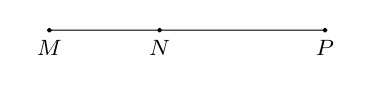
\begin{tikzpicture}[scale=0.7,line join=round,line cap=round,font=\footnotesize,>=stealth]
				\draw[fill = black] (0,0) circle(1pt) node[below]{$M$} 
				-- (2,0) circle(1pt) node[below]{$N$}
				-- (5,0) circle(1pt) node[below]{$P$}
				;	
			\end{tikzpicture}
		\end{center}
		Nhìn vào hình vẽ ta thấy cặp véc-tơ cùng hướng là $\vec{MN}$ và $\vec{MP}$.
	}
\end{ex}

\begin{ex}%NB%[0H5N1-3]
	Cho lục giác đều $ABCDEF$ tâm $O$. Véc-tơ bằng véc-tơ $\vec{AB}$ là 
	\choice
	{$\vec{DE}$}
	{$\vec{CO}$}
	{\True $\vec{FO}$}
	{$\vec{AC}$}
	\loigiai{
		\immini
		{
			Do $ABCDEF$ là lục giác đều nên $FO\parallel AB$ và $FO=AB$. \\
			Suy ra $\vec{FO} = \vec{AB}$.  
		}
		{
			\begin{tikzpicture}[line join=round, line cap = round, >=stealth, scale=.8,font=\footnotesize,transform shape]
				\foreach \x/\z/\g in
				{
					A/180/180, B/120/135,C/60/45, D/0/0,E/-60/-45,F/-120/-135
				}
				\draw[fill=black] ($(0,0)+(\z:3)$) circle(1pt) coordinate (\x) ($(\x)+(\g:3.5mm)$) node{$\x$};
				\draw[fill = black] (0,0) circle(1pt) node[below]{$O$};
				\draw
				(A)--(B)--(C)--(D)--(E)--(F)--(A)
				(A)--(D) (B)--(E) (C)--(F)
				;
			\end{tikzpicture}
		}	
	}
\end{ex}

\begin{ex}%[0H5N1-4]
	Cho đoạn thẳng $AB$ có trung điểm $M$. Véc-tơ đối của véc-tơ $\vec{AM}$ là
	\choice
	{$\vec{AM}$}
	{$\vec{MB}$}
	{$\vec{AB}$}
	{\True $\vec{BM}$}
	\loigiai{
		\begin{center}
			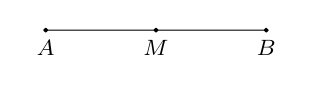
\begin{tikzpicture}[scale=0.7,line join=round,line cap=round,font=\footnotesize,>=stealth]
				\draw[fill = black] (0,0) circle(1pt) node[below]{$A$} 
				-- (2,0) circle(1pt) node[below]{$M$}
				-- (4,0) circle(1pt) node[below]{$B$}
				;	
			\end{tikzpicture}
		\end{center}
		Hai véc-tơ đối nhau là hai véc-tơ cùng độ dài và ngược hướng nên nhìn vào hình vẽ ta thấy véc-tơ cùng độ dài và ngược hướng với véc-tơ $\vec{AM}$ là $\vec{BM}$.
	}
\end{ex}

\begin{ex}%[0H5N1-1]
	Cho tứ giác $ABCD$. Số véc-tơ-không nhận các đỉnh của tứ giác làm điểm đầu và điểm cuối là
	\choice
	{$2$}
	{$6$}
	{\True $4$}
	{$12$} 
	\loigiai{
		Cứ mỗi đỉnh sẽ tạo thành một véc-tơ-không nên có tất cả $4$ véc-tơ-không nhận các đỉnh của tứ giác làm điểm đầu và điểm cuối.	
	}
\end{ex}

\begin{ex}%[0H5H1-5]
	Cho hình chữ nhật $ABCD$ có $M$, $N$ lần lượt là trung điểm $AB$, $BC$. Giá trị $k$ thoả mãn $\left|\vec{BD}\right| = k\left| \vec{MN} \right|$ là 
	\choice
	{$1$}
	{\True $2$}
	{$3$}
	{Không tồn tại}
	\loigiai{
		\immini
		{
			Ta có $MN$ là đường trung bình của tam giác $BAC$ nên 
			\[
			\left| \vec{MN} \right| = MN = \dfrac{1}{2} AC = \dfrac{1}{2}BD = \dfrac{1}{2} \left| \vec{BD} \right|.
			\]
			Vậy $k=2$.
		}
		{
			\begin{tikzpicture}[line join=round, line cap = round, >=stealth, scale=.8,font=\footnotesize,transform shape]
				\foreach \x/\y/\z/\g in
				{
					0/3/A/135, 4/3/B/45,2/3/M/90, 4/0/C/-45, 4/1.5/N/0, 0/0/D/-135
				}
				\draw[fill=black] (\x,\y) circle(1pt) coordinate (\z) ($(\z)+(\g:3.5mm)$) node{$\z$};
				\draw (C)--(A)--(B)--(C)--(D)--(A);
				\draw[->] (B)--(D);
				\draw[->] (M)--(N);
			\end{tikzpicture}
		}
	}
\end{ex}

\begin{ex}%[0H5H1-5]
	Cho tam giác $ABC$ đều cạnh $2a$ và $M$ là trung điểm $BC$. Độ dài của véc-tơ $\vec{AM}$ là 
	\choice
	{$\dfrac{a\sqrt{3}}{2}$}
	{\True $a\sqrt{3}$}
	{$2a$}
	{$a$}
	\loigiai{
		\immini
		{
			Ta có $\left| \vec{AM} \right| = AM = \sqrt{AB^2 - AM^2} = a\sqrt{3}$.
		}
		{
			\begin{tikzpicture}[line join=round, line cap = round, >=stealth, scale=.8,font=\footnotesize,transform shape]
				\foreach \x/\y/\z/\g in
				{
					0/0/B/-135, 4/0/C/-45, 2/0/M/-90, 2/3.5/A/90
				}
				\draw[fill=black] (\x,\y) circle(1pt) coordinate (\z) ($(\z)+(\g:3.5mm)$) node{$\z$};
				\draw (A)--(B)--(C)--(A);
				\draw[->] (A)--(M);
			\end{tikzpicture}
		}
	}
\end{ex}

\Closesolutionfile{ans}
\indapan{6}{ans/ans-0-C4B1.D1}
\cauds
\Opensolutionfile{ans}[ans/ans-0-C4B1.D1-DS]

\begin{ex}%[0H5N1-4]
	Xét tính Đúng/Sai của các mệnh đề sau.
	\choiceTF
	{\True Hai véc-tơ đối nhau khi chúng ngược hướng và cùng độ dài}
	{Hai véc-tơ bằng nhau khi chúng cùng phương và cùng độ dài}
	{Hai véc-tơ-không chỉ bằng nhau khi chúng cùng hướng}
	{\True Véc-tơ-không cùng phương với mọi véc-tơ}
	\loigiai{
		\begin{itemchoice}
			\itemch Đúng.
			\itemch Sai vì cùng phương chưa đủ, phải cùng hướng.
			\itemch Sai vì hai véc-tơ-không luôn bằng nhau.
			\itemch Đúng.
		\end{itemchoice}
	}
\end{ex}

\begin{ex}%[0H5H1-3]
	CHo tam giác $ABC$ có $M$, $N$ lần lượt là trung điểm của $AB$ và $AC$. Lấy $P$ đối xứng với $M$ qua $N$. Xét tính Đúng/Sai của các mệnh đề sau.
	\choiceTF
	{$MN = BC$}
	{\True $\left| \vec{MP} \right| = \left| \vec{BC} \right|$}
	{$\vec{MN}$ và $\vec{BC}$ ngược hướng}
	{\True $\vec{MP} = \vec{BC}$}
	\loigiai{
		\immini
		{
			Ta có $MN$ là đường trung bình của tam giác $ABC$ nên $MN = \dfrac{1}{2}BC$ và $MN\parallel BC$.\\
			Do đó $MP = BC$ và $MP\parallel BC$. Vậy
			\begin{itemchoice}
				\itemch Sai.
				\itemch Đúng vì $\left| \vec{MP} \right| = MP = BC = \left| \vec{BC} \right|$.
				\itemch Sai vì $\vec{MN}$ và $\vec{BC}$ cùng hướng.
				\itemch Đúng vì $\left| \vec{MP} \right| = MP = BC = \left| \vec{BC} \right|$ và $\vec{MP}$, $\vec{BC}$ cùng hướng.
			\end{itemchoice}	
		}
		{
			\begin{tikzpicture}[line join=round, line cap = round, >=stealth, scale=.8,font=\footnotesize,transform shape]
				\foreach \x/\y/\z/\g in
				{
					0/0/B/-135, 2/4/A/90, 6/0/C/-45, 1/2/M/135, 4/2/N/60, 7/2/P/45
				}
				\draw[fill=black] (\x,\y) circle(1pt) coordinate (\z) ($(\z)+(\g:3.5mm)$) node{$\z$};
				\draw (B)--(A)--(C);
				\draw[->] (M)--(P);
				\draw[->] (M)--(N);
				\draw[->] (B)--(C);
			\end{tikzpicture}
		}
	}
\end{ex}

\begin{ex}%[0H5H1-2]
	Cho tam giác $ABC$ có $M$, $N$, $P$ lần lượt là trung điểm $BC$, $CA$, $AB$. Xét tính Đúng/Sai của các mệnh đề sau.
	\choiceTF
	{\True $\vec{AB}$ và $\vec{MN}$ cùng phương}
	{Số véc-tơ khác véc-tơ-không, cùng phương với $\vec{AB}$ (không tính $\vec{AB}$) có điểm đầu, điểm cuối lấy từ các điểm đã cho là $6$}
	{$\vec{AP}$ và $\vec{PB}$ ngược hướng}
	{\True Số véc-tơ khác véc-tơ-không, cùng hướng với $\vec{BC}$ (không tính $\vec{BC}$) có điểm đầu, điểm cuối lấy từ các điểm đã cho là $3$}
	\loigiai{
		\immini
		{
			Ta có 
			\begin{itemchoice}
				\itemch Đúng vì $MN\parallel AB$.
				\itemch Sai vì có $7$ véc-tơ khác véc-tơ-không, cùng phương với $\vec{AB}$ (không tính $\vec{AB}$) có điểm đầu, điểm cuối lấy từ các điểm đã cho, cụ thể là $\vec{AP}$, $\vec{PA}$, $\vec{BA}$, $\vec{BP}$, $\vec{PB}$, $\vec{NM}$, $\vec{MN}$.
				\itemch Sai vì $\vec{AP}$ và $\vec{PB}$ cùng hướng.
				\itemch Đúng vì có $3$ véc-tơ khác véc-tơ-không, cùng hướng với $\vec{BC}$ (không tính $\vec{BC}$) có điểm đầu, điểm cuối lấy từ các điểm đã cho, cụ thể là $\vec{a}$.
			\end{itemchoice}
		}
		{
			\begin{tikzpicture}[line join=round, line cap = round, >=stealth, scale=.7,font=\footnotesize,transform shape]
				\foreach \x/\y/\z/\g in
				{
					0/0/B/-135, 2/4/A/90, 6/0/C/-45, 1/2/P/135, 4/2/N/60, 3/0/M/-90
				}
				\draw[fill=black] (\x,\y) circle(1pt) coordinate (\z) ($(\z)+(\g:3.5mm)$) node{$\z$};
				\draw (A)--(C);
				\draw[->] (A)--(B);
				\draw[->] (M)--(N);
				\draw[->] (A)--(P);
				\draw[->] (P)--(B);
				\draw[->] (B)--(C);
			\end{tikzpicture}
		}
	}
\end{ex}

\begin{ex}%[0H5V1-5]
	Cho tam giác $ABC$ nhọn có trực tâm $H$ và tâm đường tròn nội tiếp $O$. Lấy $D$ là điểm đối xứng với $A$ qua $O$. Gọi $M$ là trung điểm $BC$. Xét tính Đúng/Sai của các mệnh đề sau.
	\choiceTF
	{\True $\vec{AH}$ và $\vec{OM}$ cùng hướng}
	{$\vec{BH} = \vec{CD}$}
	{\True $\left| \vec{AH} \right| = 2\left| \vec{MO}\right|$}
	{\True $G$ là trọng tâm tam giác $AHD$}
	\loigiai{
		\immini
		{
			Do $OB=OC$ nên $OM\perp BC$ hay $OM\parallel AH$.\\
			Do $AD$ là đường kính của đường tròn $(O)$ nên $\widehat{ABD} = \widehat{ACD} = 90^\circ$.\\
			Suy ra $BD\parallel CH$, $CD\parallel BH$ hay $BDCH$ là hình bình hành.\\
			Kết hợp với $M$ là trung điểm $BC$ ta thu được $M$ là trung điểm $DH$.
		}
		{
			\begin{tikzpicture}[line join=round, line cap = round, >=stealth, scale=.8,font=\footnotesize,transform shape]
				\foreach \x/\y/\z/\g in
				{
					0/0/O/170, -2/3/A/90, 3/-2/C/-45, -3/-2/B/-135, 0/-2/M/-135, 2/-3/D/-90, -2/-1/H/135
				}
				\draw[fill=black] (\x,\y) circle(1pt) coordinate (\z) ($(\z)+(\g:3.5mm)$) node{$\z$};
				\pgfmathsetmacro\rr{sqrt(13)}
				\draw [fill=black] (intersection of H--O and A--M) circle(1pt) node[left]{$G$}; 
				\draw (A)--(B)--(D)--(C)--(A)--(H)--(D)--(A) (H)--(B)--(C)--(H) (H)--(O)--(M)--(A);
				\draw (O) circle(\rr);
			\end{tikzpicture}
		}
		Vậy
		\begin{itemchoice}
			\itemch Đúng vì $OM\parallel AH$.
			\itemch Sai vì $\vec{BH}$ và $\vec{CD}$ ngược hướng và cùng độ dài khác $0$ nên chúng đối nhau chứ không bằng nhau.
			\itemch Đúng vì $OM$ là đường trung bình của tam giác $ADH$ nên $AH =2OM$ hay $\left| \vec{AH} \right| = AH = 2OM = 2\left| \vec{MO}\right|$.
			\itemch Đúng vì $G$ thuộc trung tuyến $AM$ của tam giác $AHD$ và $AG=2GM$.
		\end{itemchoice}
	}
\end{ex}

\Closesolutionfile{ans}
\indapan{3}{ans/ans-0-C4B1.D1-DS}

\Opensolutionfile{ans}[ans/ans-0-C4B1.D1-KQ]
\caukq
\begin{ex}%[0H5N1-1]
	Ta tạo được bao nhiêu véc-tơ khác véc-tơ-không có điểm đầu và điểm cuối nằm trong $4$ điểm phân biệt cho trước trên mặt phẳng?
	\shortans{$12$}
	\loigiai{
		Chọn điểm đầu có $4$ cách, sau đó ta chọn điểm cuối trong $3$ điểm khác điểm đầu nên ta tạo được $3\cdot 4 = 12$ véc-tơ.
	}
\end{ex}

\begin{ex}%[0H5H1-5]
	Cho véc-tơ $\vec{AB}$ khác véc-tơ-không và điểm $C$ không nằm trên đường thẳng $AB$. Có bao nhiêu điểm $D$ thoả mãn $\left| \vec{CD} \right| = \left| \vec{AB} \right|$ và hai đường thẳng $AB$, $CD$ không cắt nhau.
	\shortans{$2$}
	\loigiai{
		Hai đường thẳng $AB$, $CD$ không cắt nhau nên $D$ thuộc đường thẳng qua $C$ song song với $AB$, gọi là đường thẳng $\Delta$.\\
		Lại có 	$\left| \vec{CD} \right| = \left| \vec{AB} \right|$ nên $AB=CD$ hay $D$ thuộc đường tròn tâm $C$ bán kính $AB$, gọi là đường tròn $(C)$.\\
		Đường thẳng $\Delta$ cắt đường tròn $(C)$ tại hai điểm nên có $2$ điểm $D$ thoả mãn.
	}
\end{ex}

\begin{ex}%[0H5H1-3]
	Cho lục giác đều $ABCDEF$ tâm $O$. Có bao nhiêu véc-tơ bằng véc-tơ $\vec{OD}$ có điểm đầu và điểm cuối là các điểm trong hình (không tính $\vec{OD}$)? 
	\shortans{$3$}
	\loigiai{
		\immini
		{
			Do $ABCDEF$ là lục giác đều nên $AO = OD = BC = FE$ và $BC\parallel AD\parallel FE$.  \\
			Vậy $\vec{BC} = \vec{AO} = \vec{FE} = \vec{OD}$.
		}
		{
			\begin{tikzpicture}[line join=round, line cap = round, >=stealth, scale=.8,font=\footnotesize,transform shape]
				\foreach \x/\z/\g in
				{
					A/180/180, B/120/135,C/60/45, D/0/0,E/-60/-45,F/-120/-135
				}
				\draw[fill=black] ($(0,0)+(\z:3)$) circle(1pt) coordinate (\x) ($(\x)+(\g:3.5mm)$) node{$\x$};
				\draw[fill = black] (0,0) circle(1pt) node[below]{$O$};
				\draw
				(A)--(B)--(C)--(D)--(E)--(F)--(A)
				(A)--(D) (B)--(E) (C)--(F)
				;
			\end{tikzpicture}
		}	
	}
\end{ex}

\begin{ex}%[0H5H1-5]
	Cho hình thoi $ABCD$ có $\widehat{BAD} = 60^\circ$ và $AB = 2\sqrt{3}$. Tính độ dài của véc-tơ $\vec{AC}$.
	\shortans{$6$}
	\loigiai{
		\immini
		{
			Gọi $O$ là giao điểm của $AC$ và $BD$. Khi đó do $ABCD$ là hình thoi nên $AO\perp BD$ và $AC = 2AO$.\\
			Do $AB = AD$ và $\widehat{BAD} = 60^\circ$ nên $BAD$ là tam giác đều cạnh $2\sqrt{3}$.\\
			Suy ra $AO = 2\sqrt{3} \cdot \sin 60^\circ = 3$.\\
			Vậy $\left| \vec{AC} \right| = AC = 2AO = 6$.
		}
		{
			\begin{tikzpicture}[line join=round, line cap = round, >=stealth, scale=.8,font=\footnotesize,transform shape]
				\foreach \x/\y/\z/\g in
				{
					0/0/O/-45, -3.5/0/A/180, 0/2/B/90, 3.5/0/C/0,0/-2/D/-90
				}
				\draw[fill=black] (\x,\y) circle(1pt) coordinate (\z) ($(\z)+(\g:3.5mm)$) node{$\z$};
				\draw (A)--(B)--(C)--(D)--(A)--(C) (B)--(D);
			\end{tikzpicture}
		}
	}
\end{ex}

\begin{ex}%[0H5H1-5]
	Cho hình vuông $ABCD$ cạnh $2$ có $M$ là trung điểm $AB$, $N$ là điểm đối xứng với $D$ qua $C$. Tính độ dài véc-tơ $\vec{MN}$ (làm tròn đến chữ số thập phân thứ hai sau dấu phẩy).
	\shortans{$3{,}61$}
	\loigiai{
		\immini
		{
			Gọi $E$ là trung điểm cạnh $CD$. \\
			Khi đó $ME\perp CD$ và $MN = AD = 2$, $EN = \dfrac{3}{2}CD = 3$.\\
			Suy ra $\left| \vec{MN} \right| = MN = \sqrt{ME^2 + EN^2} = \sqrt{13} \approx 3{,}61$.
		}
		{
			\begin{tikzpicture}[line join=round, line cap = round, >=stealth, scale=.8,font=\footnotesize,transform shape]
				\foreach \x/\y/\z/\g in
				{
					0/2/A/135, 2/2/B/45, 2/0/C/-90, 0/0/D/-135, 4/0/N/-45, 1/0/E/-90, 1/2/M/90
				}
				\draw[fill=black] (\x,\y) circle(1pt) coordinate (\z) ($(\z)+(\g:3.5mm)$) node{$\z$};
				\draw (E)--(M)--(N)--(D)--(A)--(B)--(C);
			\end{tikzpicture}
		}
	}
\end{ex}

\begin{ex}%[0H5V1-3]
	Số cặp véc-tơ khác véc-tơ-không và bằng nhau nhiều nhất tạo được từ $4$ điểm phân biệt nhiều nhất là bao nhiêu?
	\shortans{$8$}
	\loigiai{
		\begin{center}
			\begin{tikzpicture}[line join=round, line cap = round, >=stealth, scale=.8,font=\footnotesize,transform shape]
				\foreach \x/\y/\z/\g in
				{
					0/0/A/-90, 2/0/B/-90, 4/0/C/-90, 6/0/D/-90
				}
				\draw[fill=black] (\x,\y) circle(1pt) coordinate (\z) ($(\z)+(\g:3.5mm)$) node{$\z$};
				\draw (A)--(B)--(C)--(D);
			\end{tikzpicture}
		\end{center}
		Gọi $4$ điểm phân biệt là $A$, $B$, $C$, $D$.\\
		Để tạo ra nhiều cặp véc-tơ khác véc-tơ-không và bằng nhau nhiều nhất từ $4$ điểm phân biệt thì ta xếp $4$ điểm $A$, $B$, $C$, $D$ trên một đường thẳng thoả mãn $AB = BC = CD$.\\
		Khi đó ta tạo được $8$ cặp véc-tơ bằng nhau là $\vec{AB} = \vec{BC}$, $\vec{AB} = \vec{CD}$, $\vec{BC} = \vec{CD}$, $\vec{AC} = \vec{BD}$ và các cặp véc-tơ đối của mỗi cặp.
	}
\end{ex}
\Closesolutionfile{ans}
\indapan{6}{ans/ans-0-C4B1.D1-KQ}
\newpage 
\subsection{Đề 2}
\Opensolutionfile{ans}[ans/ans-0-B1]
\caulc
\begin{ex}%[0D1N1-2]
	Cho tứ giác $ABCD$ có $\overrightarrow{AD}=\overrightarrow{BC}$. Mệnh đề nào trong các mệnh đề sau là \textbf{sai}?
	\choice
	{Tứ giác $ABCD$ là hình bình hành}
	{$DA=BC$}
	{\True $\overrightarrow{AC}=\overrightarrow{BD}$}
	{$\overrightarrow{AB}=\overrightarrow{DC}$}
	\loigiai{
		\immini
		{$AC$ và $BD$ là hai đường chéo của tứ giác $ABCD$ nên hai véc-tơ $\overrightarrow{AC}$, $\overrightarrow{BD}$ không cùng phương vì vậy không thể bằng nhau.}
		{
			\begin{tikzpicture}[scale=1,line join=round,line cap=round,font=\footnotesize,>=stealth]
				\def\d{4}
				\def\r{3}
				\path (0:0) coordinate (B)
				++(0:\d) coordinate (C)
				++(50:\r) coordinate (D)
				($(B)+(D)-(C)$) coordinate (A);
				\draw (A)--(B)--(C)--(D)--cycle;
				\foreach \x/ \goc in {A/180,B/180,C/0,D/0} 
				\fill (\x) circle (1pt)	
				($(\x)+(\goc:3mm)$) node {$\x$};
			\end{tikzpicture}
		}
	}
\end{ex}
%Câu 2
\begin{ex}%[0D1N1-2]
	Gọi $O$ là giao điểm hai đường chéo $AC$ và $BD$ của hình bình hành $ABCD$. Đẳng thức nào sau đây là đẳng thức \textbf{sai}?
	\choice
	{$\overrightarrow{OB}=\overrightarrow{DO}$}
	{$\overrightarrow{AB}=\overrightarrow{DC}$}
	{\True $\overrightarrow{OA}=\overrightarrow{OC}$}
	{$\overrightarrow{CB}=\overrightarrow{DA}$}
	\loigiai{
		\immini
		{$\overrightarrow{OA}$ và $\overrightarrow{OC}$ là hai véc-tơ đối nhau nên không thể bằng nhau.}
		{
			\begin{tikzpicture}[scale=1,line join=round,line cap=round,font=\footnotesize,>=stealth]
				\def\d{4}
				\def\r{3}
				\path (0:0) coordinate (B)
				++(0:\d) coordinate (C)
				++(50:\r) coordinate (D)
				($(B)+(D)-(C)$) coordinate (A)
				(intersection of A--C and B--D) coordinate (O);%giao điểm O
				\draw (A)--(B)--(C)--(D)--cycle (A)--(C) (B)--(D);
				\foreach \x/ \goc in {A/180,B/180,C/0,D/0,O/80} 
				\fill (\x) circle (1pt)	
				($(\x)+(\goc:3mm)$) node {$\x$};
			\end{tikzpicture}
		}
	}
\end{ex}
%Câu 3
\begin{ex}%[0D1N1-2]
	Cho hình bình hành $ABCD$ tâm $O$. Gọi $P$, $Q$, $R$ lần lượt là trung điểm của $AB$, $BC$, $AD$. Tìm mệnh đề \textbf{sai}?
	\choice
	{Có $2$ véc-tơ bằng $\overrightarrow{PR}$}
	{Có $4$ véc-tơ bằng $\overrightarrow{AR}$}
	{Có $2$ véc-tơ bằng $\overrightarrow{BO}$}
	{\True Có 5 véc-tơ bằng $\overrightarrow{OP}$}
	\loigiai{
		\immini
		{Ta có
			\begin{eqnarray*}
				&&\overrightarrow{PQ}=\overrightarrow{AO}=\overrightarrow{OC}.\\
				&&\overrightarrow{AR}=\overrightarrow{RQ}=\overrightarrow{PO}=\overrightarrow{BQ}=\overrightarrow{QC}.\\
				&&\overrightarrow{BO}=\overrightarrow{OD}=\overrightarrow{PR}.\\
				&&\overrightarrow{OP}=\overrightarrow{RA}=\overrightarrow{DR}=\overrightarrow{CQ}=\overrightarrow{QB}.
		\end{eqnarray*}}
		{
			\begin{tikzpicture}[scale=1,line join=round,line cap=round,font=\footnotesize,>=stealth]
				\def\d{4}
				\def\r{3}
				\path (0:0) coordinate (B)
				++(0:\d) coordinate (C)
				++(50:\r) coordinate (D)
				($(B)+(D)-(C)$) coordinate (A)
				(intersection of A--C and B--D) coordinate (O)  %giao điểm O
				($(A)!0.5!(B)$) coordinate (P)
				($(B)!0.5!(C)$) coordinate (Q)
				($(A)!0.5!(D)$) coordinate (R);
				\draw (A)--(B)--(C)--(D)--cycle (A)--(C) (B)--(D) (P)--(R) (O)--(P);
				\foreach \x/ \goc in {A/180,B/180,C/0,D/0,O/80,P/180,Q/-90,R/90} 
				\fill (\x) circle (1pt)	
				($(\x)+(\goc:3mm)$) node {$\x$};
			\end{tikzpicture}
		}
	}
\end{ex}
%Câu 4
\begin{ex}%[0D1H1-2]
	Cho hình chữ nhật $ABCD$ có $AB=3$, $BC=4$. Tính độ dài của véc-tơ $\overrightarrow{CA}$.
	\choice
	{\True $\left|\overrightarrow{CA}\right|=5$}
	{$\left|\overrightarrow{CA}\right|=25$}
	{$\left|\overrightarrow{CA}\right|=7$}
	{$\left|\overrightarrow{CA}\right|=\sqrt 7 $}
	\loigiai{
		\immini
		{Xét tam giác $ABC$ vuông tại $B$, ta có\\ $\left|\overrightarrow{CA}\right|=CA=\sqrt{AB^2+BC^2}=5$.}
		{
			\begin{tikzpicture}[scale=1,line join=round,line cap=round,font=\footnotesize,>=stealth]
				\def\d{4} %dài
				\def\r{3} %rộng
				\path 	(0:0) coordinate (B)
				++(0:\d) coordinate (C)
				++(90:\r) coordinate (D)
				++(180:\d) coordinate (A);
				\draw (A)--(B)--(C)--(D)--cycle (C)--(A);
				\foreach \x/ \goc in {A/135,B/-135,C/-45,D/45} 
				\fill (\x) circle (1pt)
				($(\x)+(\goc:3mm)$) node {$\x$};
			\end{tikzpicture}
		}
	}
\end{ex}
%Câu 5
\begin{ex}%[0D1H1-2]
	Cho tam giác $ABC$ đều cạnh $2a$. Gọi $M$ là trung điểm $BC$. Khi đó $\left|\overrightarrow{AM}\right|$ bằng
	\choice
	{$2a$}
	{$2a\sqrt 3 $}
	{$4a$}
	{\True $a\sqrt 3 $}
	\loigiai{
		\immini
		{Xét tam giác $ABM$ vuông tại $M$, ta có\\ $\left|\overrightarrow{AM}\right|=AM=\sqrt{A{B^2}-B{M^2}}\\
			=\sqrt{(2a)^2-a^2}\\
			=a\sqrt 3$.}
		{
			\begin{tikzpicture}[scale=1,line join=round,line cap=round,font=\footnotesize,>=stealth]
				\def\a{3}
				\path (0:0) coordinate (B)
				++(0:\a) coordinate (C)	
				([turn]120:\a) coordinate (A)
				($(B)!0.5!(C)$) coordinate (M);
				\draw (A)--(B)--(C)--cycle;
				\foreach \x/ \goc in {A/135,B/-135,C/-45,M/-90} 
				\fill (\x) circle (1pt)
				($(\x)+(\goc:3mm)$) node {$\x$};	
			\end{tikzpicture}
		}
	}
\end{ex}
%Câu 6
\begin{ex}%[0D1H1-2]
	Cho hình thoi tâm $O$, cạnh bằng $a$ và $\widehat A=60^\circ $. Kết luận nào sau đây là \textbf{đúng}?
	\choice
	{\True $\left|\overrightarrow{AO}\right|=\dfrac{a\sqrt 3}{2}$}
	{$\left|\overrightarrow{OA}\right|=a$}
	{$\left|\overrightarrow{OA}\right|=\left|\overrightarrow{OB}\right|$}
	{$\left|\overrightarrow{OA}\right|=\dfrac{a\sqrt 2}{2}$}
	\loigiai{
		\immini
		{Vì $\widehat A=60^\circ\Rightarrow\Delta ABC$ đều $\Rightarrow AO=\dfrac{a\sqrt 3}{2}\Rightarrow\left|\overrightarrow{AO}\right|=\dfrac{a\sqrt3}{2}$.}
		{
			\begin{tikzpicture}[scale=1,line join=round,line cap=round,font=\footnotesize,>=stealth]
				\def\a{3} %cạnh
				\path 	(0:0) coordinate (B)
				++(30:\a) coordinate (C)
				++(150:\a) coordinate (D)
				++(210:\a) coordinate (A)
				(intersection of A--C and B--D) coordinate (O);
				\draw (A)--(B)--(C)--(D)--cycle (A)--(C) (B)--(D);
				\foreach \x/ \goc in {A/180,B/-90,C/0,D/90,O/45} 
				\fill (\x) circle (1pt)
				($(\x)+(\goc:3mm)$) node {$\x$};
			\end{tikzpicture}
		}
	}
\end{ex}
%Câu 7
\begin{ex}%[0D1H1-2]
	Cho tam giác không cân $ABC$. Gọi $H$, $O$ lần lượt là trực tâm, tâm đường tròn ngoại tiếp của tam giác, $M$ là trung điểm của $BC$. Mệnh đề nào sau đây là \textbf{đúng}?
	\choice
	{\True Tam giác $ABC$ nhọn thì $\overrightarrow{AH}$, $\overrightarrow{OM}$ cùng hướng}
	{$\overrightarrow{AH}$, $\overrightarrow{OM}$ luôn cùng hướng}
	{$\overrightarrow{AH}$, $\overrightarrow{OM}$ cùng phương nhưng ngược hướng}
	{$\overrightarrow{AH}$, $\overrightarrow{OM}$ có cùng giá}
	\loigiai{
		\immini
		{Thật vậy khi $\Delta ABC$ nhọn thì ta có\\
			$\heva{AH\perp BC\\
				OM\perp BC}
			\Rightarrow AH \parallel OM$.\\
			$O$, $H$ nằm trong tam giác $\Rightarrow\overrightarrow{AH}$, $\overrightarrow{OM}$ cùng hướng.}
		{
			\begin{tikzpicture}[scale=1,line join=round,line cap=round,font=\footnotesize,>=stealth]
				\path 
				(-2,3) coordinate (A)
				(-3,-1) coordinate (B)
				(4,-1) coordinate (C)
				(1/2,1/4) coordinate (O);
				\coordinate (P) at ($(B)!(A)!(C)$);
				\coordinate (N) at ($(A)!(B)!(C)$);	
				\coordinate (H) at (intersection of A--P and B--N);
				\coordinate (M) at ($(B)!0.5!(C)$);
				\coordinate (Q) at ($(A)!0.5!(C)$);
				%\draw[step=1,gray!50,very thin] (-5,-5) grid (5,5);
				%	\draw[->] (-5,0)--(5,0) node[below] { $x$};
				%	\draw[->] (0,-5)--(0,5) node[left] { $y$};
				%	\draw (0,0) node [below left] { $W$};
				\draw[->] (A)--(H) (O)--(M);
				\draw (A)--(B)--(C)--cycle (A)--(P) (B)--(N) (Q)--(O)
				pic[draw,angle radius=2mm]{right angle=A--P--C} pic[draw,angle radius=2mm]{right angle=A--N--B}		pic[draw,angle radius=2mm]{right angle=A--Q--O} pic[draw,angle radius=2mm]{right angle=C--M--O};
				\foreach \x/ \goc in {A/135,B/-135,C/-45,P/-90,N/30,H/0,M/-90,Q/30,O/0} 
				\fill (\x) circle (1pt)
				($(\x)+(\goc:3mm)$) node {$\x$};
			\end{tikzpicture}
		}
	}
\end{ex}
%Câu 8
\begin{ex}%[0D1H1-2]
	Cho đường tròn tâm $O$. Từ điểm $A$ nằm ngoài $(O)$, kẻ hai tiếp tuyến $AB$, $AC$ tới $(O)$.\\
	Xét mệnh đề:\\
	(I) $\overrightarrow{AB}=\overrightarrow{AC}$\\
	(II) $\overrightarrow{OB}=-\overrightarrow{OC}$\\
	(III) $\left|\overrightarrow{BO}\right|=\left|\overrightarrow{CO}\right|$\\
	Mệnh đề \textbf{đúng} là:
	\choice
	{Chỉ (I)}
	{(I) và (III)}
	{(I), (II), (III)}
	{\True Chỉ (III)}
	\loigiai{
		Ta có $OB=OC=R\Rightarrow\left|\overrightarrow{BO}\right|=\left|\overrightarrow{CO}\right|$.
	}
\end{ex}
%Câu 9
\begin{ex}%[0D1H1-2]
	Cho tam giác $ABC$ có $H$ là trực tâm và $O$ là tâm đường tròn ngoại tiếp. Gọi $D$ là điểm đối xứng với $B$ qua $O$.
	\choice
	{\True $\overrightarrow{AH}=\overrightarrow{DC}$}
	{$\overrightarrow{AB}=\overrightarrow{DC}$}
	{$\overrightarrow{AD}=\overrightarrow{BC}$}
	{$\overrightarrow{AO}=\overrightarrow{AH}$}
	\loigiai{
		Ta có thể chỉ ra được $ADCH$ là hình bình hành $\Rightarrow\overrightarrow{AH}=\overrightarrow{DC}$.
	}
\end{ex}
%Câu 10
\begin{ex}%[0D1H1-2]
	Cho tứ giác $ABCD$. Gọi $M$, $N$, $P$ lần lượt là trung điểm của $AD$, $BC$ và $AC$. Biết $\overrightarrow{MP}=\overrightarrow{PN}$. Chọn câu \textbf{đúng}.
	\choice
	{$\overrightarrow{AC}=\overrightarrow{BD}$}
	{$\overrightarrow{AC}=\overrightarrow{BC}$}
	{\True $\overrightarrow{AD}=\overrightarrow{BC}$}
	{$\overrightarrow{AD}=\overrightarrow{BD}$}
	\loigiai{
		\begin{center}
			\begin{tikzpicture}[scale=1,line join=round,line cap=round,font=\footnotesize,>=stealth]
				\def\d{4}
				\def\r{3}
				\path (0:0) coordinate (B)
				++(0:\d) coordinate (C)
				++(70:\r) coordinate (D)
				($(B)+(D)-(C)$) coordinate (A)
				%	(intersection of A--C and B--D) coordinate (O)  %giao điểm O
				($(A)!0.5!(C)$) coordinate (P)
				($(B)!0.5!(C)$) coordinate (N)
				($(A)!0.5!(D)$) coordinate (M);
				\draw (A)--(B)--(C)--(D)--cycle (A)--(C) ;
				\foreach \x/ \goc in {A/180,B/180,C/0,D/0,M/90,N/-90,P/90} 
				\fill (\x) circle (1pt)	
				($(\x)+(\goc:3mm)$) node {$\x$};
			\end{tikzpicture}
		\end{center}
		Ta có $MP \parallel DC$, $MP=\dfrac{1}{2}DC$, $PN//AB$, $PN=\dfrac{1}{2}AB$.\\ Mà $MP=PN \Rightarrow\overrightarrow{AB}=\overrightarrow{DC}\Rightarrow ABCD$ là hình bình hành $\Rightarrow\overrightarrow{AD}=\overrightarrow{BC}$.
	}
\end{ex}
%Câu 11
\begin{ex}%[0D1N1-2]
	Cho hình lục giác đều $ABCDEF$ tâm $O$. Số các véc-tơ khác véc-tơ không, cùng phương với véc-tơ $\overrightarrow{OB}$ có điểm đầu và điểm cuối là các đỉnh của lục giác là
	\choice
	{$4$}
	{\True $6$}
	{$8$}
	{$10$}
	\loigiai{
		\begin{center}
			\begin{tikzpicture}[scale=1,line join=round,line cap=round,font=\footnotesize,>=stealth]
				\def\a{2}
				\path (0:0) coordinate (O)
				(0:\a) coordinate (C)	
				(60:\a) coordinate (D)
				(120:\a) coordinate (E)
				(180:\a) coordinate (F)
				(240:\a) coordinate (A)
				(300:\a) coordinate (B);
				\draw (A)--(B)--(C)--(D)--(E)--(F)--(A) (O)--(B);
				\foreach \x/ \goc in {A/180,B/-135,C/-45,D/0,E/90,F/180,O/0} 
				\fill (\x) circle (1pt)
				($(\x)+(\goc:3mm)$) node {$\x$};	
			\end{tikzpicture}
		\end{center}
		Các véc-tơ cùng phương với véc-tơ $\overrightarrow{OB}$ là\\
		$\overrightarrow{BE}$, $\overrightarrow{EB}$, $\overrightarrow{DC}$, $\overrightarrow{CD}$, $\overrightarrow{FA}$, $\overrightarrow{AF}$.
	}
\end{ex}
%Câu 12
\begin{ex}%[0D1H1-2]
	Cho $\Delta ABC$ với điểm $M$ nằm trong tam giác. Gọi $A'$, $B'$, $C'$ lần lượt là trung điểm của $BC$, $CA$, $AB$ và $N$, $P$, $Q$ lần lượt là các điểm đối xứng với $M$ qua $A'$, $B'$, $C'$. 
	\choice
	{$\overrightarrow{AM}=\overrightarrow{PC}$ và $\overrightarrow{QB}=\overrightarrow{NC}$}
	{\True $\overrightarrow{AC}=\overrightarrow{QN}$ và $\overrightarrow{AM}=\overrightarrow{PC}$}
	{$\overrightarrow{AB}=\overrightarrow{CN}$ và $\overrightarrow{AP}=\overrightarrow{QN}$}
	{$\overrightarrow{AB'}=\overrightarrow{BN}$ và $\overrightarrow{MN}=\overrightarrow{BC}$}
	\loigiai{
		Ta có $AMCP$ là hình bình hành $\Rightarrow\overrightarrow{AM}=\overrightarrow{PC}$\\
		Ta lại có $AQBM$ và $BMCN$ là hình bình hành\\
		$\Rightarrow NC=BM=QA$\\
		$\Rightarrow AQNC$ là hình bình hành $\Rightarrow\overrightarrow{AC}=\overrightarrow{QN}$.
	}
\end{ex}


\Closesolutionfile{ans}
\indapan{6}{ans/ans-0-B1}
\cauds
\Opensolutionfile{ans}[ans/ans-0-B1-DS]
%Câu 1
\begin{ex}%[0D1N1-2]
	Cho tứ giác $ABCD$. Khi đó
	\choiceTF
	{Có 5 véc-tơ có điểm đầu hoặc điểm cuối là điểm $A$}
	{\True Có 4 véc-tơ có điểm đầu hoặc điểm cuối là điểm $B$ mà không có điểm đầu hoặc điểm cuối là điểm $A$}
	{\True Có 2 véc-tơ có điểm đầu và điểm cuối là các điểm $C$, $D$}
	{Có 10 véc-tơ (khác $\vec 0$) có điểm đầu và điểm cuối là các điểm $A$, $B$, $C$, $D$}
	\loigiai{
		\immini
		{	\begin{itemchoice}
				\itemch Sai. Vì có 6 véc-tơ liên quan đến điểm $A$ là $\overrightarrow{AB}$, $\overrightarrow{BA}$, $\overrightarrow{AC}$, $\overrightarrow{CA}$, $\overrightarrow{AD}$, $\overrightarrow{DA}$.
				\itemch Đúng. Vì có 4 véc-tơ liên quan đến điểm $B$ mà không liên quan đến $A$ là $\overrightarrow{BC}$, $\overrightarrow{CB}$, $\overrightarrow{BD}$, $\overrightarrow{DB}$.
				\itemch Đúng. Vì có 2 véc-tơ liên quan đến hai điểm $C$, $D$ là $\overrightarrow{CD}$, $\overrightarrow{DC}$.
				\itemch Sai. Vì có 12 véc-tơ (khác $\vec 0$) có điểm đầu và điểm cuối là các điểm $A$, $B$, $C$, $D$.
			\end{itemchoice}
		}
		{	\begin{tikzpicture}[scale=1,line join=round,line cap=round,font=\footnotesize,>=stealth]
				\def\a{3}
				\path (0:0) coordinate (A)
				(0:\a) coordinate (B)	
				(60:\a*1.5) coordinate (C)
				(120:\a) coordinate (D);
				\draw (A)--(B)--(C)--(D)--(A);
				\foreach \x/ \goc in {A/180,B/-90,C/0,D/180} 
				\fill (\x) circle (1pt)
				($(\x)+(\goc:3mm)$) node {$\x$};
			\end{tikzpicture}
		}
	}
\end{ex}
%Câu 2
\begin{ex}%[0D1H1-2]
	Cho $\Delta ABC$ có $A^\prime$, $B^\prime$, $C^\prime$ lần lượt là các trung điểm của các cạnh $BC$, $CA$, $AB$. Khi đó
	\choiceTF
	{\True $B{C^\prime}=C^\prime A=A^\prime{B^\prime}=\dfrac{AB}{2}{\rm}$}
	{Hai véc-tơ $\overrightarrow{B{C^\prime}},\overrightarrow{A^\prime{B^\prime}}$ ngược hướng}
	{\True $\overrightarrow{B{C^\prime}}=\overrightarrow{C^\prime A} =\overrightarrow{A^\prime{B^\prime}}$}
	{\True $\overrightarrow{B^\prime C^\prime}=\overrightarrow{CA^\prime}$}
	\loigiai{
		\begin{center}
			\begin{tikzpicture}[scale=1,line join=round,line cap=round,font=\footnotesize,>=stealth]
				\def\r{3}
				\path 	(180:\r) coordinate (B)
				(0:\r) coordinate (C)	
				(120:\r) coordinate (A)
				($(B)!0.5!(C)$) coordinate (A')
				($(C)!0.5!(A)$) coordinate (B')
				($(B)!0.5!(A)$) coordinate (C');
				\draw (A)--(B)--(C)--cycle;
				\foreach \x/ \goc in {A/135,B/-135,C/-45,A'/-90,B'/30,C'/180} 
				\fill (\x) circle (1pt)
				($(\x)+(\goc:3mm)$) node {$\x$};	
			\end{tikzpicture}
		\end{center}
		\begin{itemchoice}
			\itemch Đúng. Ta có $C^\prime$ là trung điểm của $AB$ và $A^\prime{B^\prime}$ là đường trung bình của tam giác $ABC$ ứng với cạnh đáy $AB$ nên $B{C^\prime}=C^\prime A=A^\prime{B^\prime}=\dfrac{AB}{2}$.
			\itemch Sai. Vì Hai véc-tơ $\overrightarrow{B{C^\prime}},\overrightarrow{A^\prime{B^\prime}}$ cùng hướng.
			\itemch Đúng. Vì $C^\prime$ là trung điểm của $AB$ và $A^\prime{B^\prime}$ là đường trung bình của tam giác $ABC$ ứng với cạnh đáy $AB$ nên  $\overrightarrow{B{C^\prime}}=\overrightarrow{C^\prime A} =\overrightarrow{A^\prime{B^\prime}}$.
			\itemch Đúng. Vì $A^\prime$ là trung điểm của $BC$ và $B^\prime{C^\prime}$ là đường trung bình của tam giác $ABC$ ứng với cạnh đáy $BC$ nên $\overrightarrow{B^\prime{C^\prime}}=\overrightarrow{C{A^\prime}}$.
		\end{itemchoice}
	}
\end{ex}
%Câu 3
\begin{ex}%[0D1V1-2]
	Cho tam giác $ABC$ vuông tại $A$ có $AB=\sqrt{3}$, $AC=2\sqrt{3}$. Gọi $M$ là trung điểm $BC$ và $H$ là hình chiếu vuông góc của $A$ lên $BC$. Khi đó
	\choiceTF
	{\True $B{C^2}=A{B^2}+A{C^2}$}
	{$|\overrightarrow{AM}|=\dfrac{\sqrt{15}}{4}$}
	{\True $AB\cdot AC=AH\cdot BC$}
	{$|\overrightarrow{AH}|=\dfrac{\sqrt{15}}{5}$}
	\loigiai{
		\begin{itemchoice}
			\itemch Đúng. Áp dụng định lý Pytago cho tam giác $ABC$ vuông tại $A$.
			\itemch Sai. Áp dụng định lí Pytago trong $\Delta ABC$ vuông tại $A$, ta có\\ $BC^2=AB^2+AC^2=\sqrt{3} ^2+(2 \sqrt{3})^2=15$\\
			$\Rightarrow \left|\overrightarrow{BC} \right| =BC=\sqrt{15}$.\\
			Ta có $AM$ là trung tuyến ứng với cạnh huyền $BC$\\
			$\Rightarrow \left| \overrightarrow{AM} \right| =AM=\dfrac{BC}{2}=\dfrac{\sqrt{15}}{2}$.
			\itemch Đúng. Vì theo hệ thức lượng trong tam giác vuông.
			\itemch Sai. Ta có $AB\cdot AC=AH\cdot BC$ (hệ thức lượng trong tam giác vuông)\\
			$\Rightarrow \left| \overrightarrow{AH} \right| =AH=\dfrac{AB\cdot AC}{BC}=\dfrac{\sqrt 3\cdot 2\sqrt 3}{\sqrt{15}}=\dfrac{2\sqrt{15}}{5}$.
		\end{itemchoice}
	}
\end{ex}
%Câu 4
\begin{ex}%[0D1V1-2]
	Cho hình thang $ABCD$ vuông tại $A$ và có $AB=AD=\dfrac{1}{2}DC=a$. Gọi $BF$ là đường phân giác trong của tam giác $ABD(F\in AD)$. Khi đó
	\choiceTF
	{\True $C{A^2}=D{A^2}+D{C^2}$}
	{$|\overrightarrow{CA}|=a\sqrt 3 $}
	{$\widehat{ABF}=45^\circ$}
	{$|\overrightarrow{BF}|\approx 2.08a$}
	\loigiai{
		\begin{itemchoice}
			\itemch Đúng. Áp dụng định lí Pytago cho tam giác $ADC$ vuông tại $D$.
			\itemch Sai. Áp dụng định lí Pytago cho tam giác $ADC$ vuông tại $D$, ta có\\
			$C{A^2}=D{A^2}+D{C^2}=a^2+(2a)^2=5a^2$\\
			$\Rightarrow |\overrightarrow{CA}|=CA=a\sqrt 5$.
			\itemch Sai. Ta có $\Delta ABD$ vuông cân tại $A$, do đó\\
			$\widehat{ABD}=45^\circ \Rightarrow \widehat{ABF}=22.5^\circ$.
			\itemch Sai. Xét $\Delta ABF$ vuông tại $A$, ta có\\
			$ \left| \overrightarrow{BF} \right| =BF=\dfrac{AB}{\cos \left( ABF \right)}=\dfrac{a}{\cos{22.5^\circ}}\approx 1.08a$.
		\end{itemchoice}
	}
\end{ex}
\Closesolutionfile{ans}
\indapan{3}{ans/ans-0-B1-DS}



\Opensolutionfile{ans}[ans/ans-0-B1-KQ]
\caukq
%Câu 1
\begin{ex}%[0D1H1-2]
	Cho tam giác $ABC$ vuông tại $A$ có $AB=3$, $AC=4$. Khi đó $\left|\overrightarrow{BC}\right|$ bằng
	\shortans{$5$}
	\loigiai{
		Áp dụng định lý Pytago vào tam giác vuông $ABC$, ta có\\
		$BC^2=AC^2+AB^2=4^2+3^2=25$\\
		$\Rightarrow BC=5$.\\
		Khi đó $\left|\overrightarrow{BC}\right|=BC=5$.
	}
\end{ex}
%Câu 2
\begin{ex}%[0D1H1-2]
	Cho hình vuông $ABCD$ cạnh bằng $1$, tâm $O$. Tính $\left|\overrightarrow{OD}\right|$.
	\shortans{$0{,}71$}
	\loigiai{
		Hình vuông $ABCD$ cạnh bằng $1$, nên $BD=\sqrt{2}$.\\
		Ta có $\left|\overrightarrow{OD}\right|=OD=\dfrac{BD}{2}=\dfrac{1 \cdot \sqrt 2}{2} \approx 0{,}71$.
	}
\end{ex}
%Câu 3
\begin{ex}%[0D1H1-2]
	Cho hình thoi $ABCD$ cạnh $2$ và $\widehat{BAD}=60^\circ$. Tìm độ dài $\overrightarrow{AC}$.
	\shortans{$3{,}46$}
	\loigiai{
		Gọi $O$ là giao điểm của hai đường chéo $AC$ và $BD$.\\
		Theo quy tắc hình bình hành, ta có $\overrightarrow{AB}+\overrightarrow{AD}=\overrightarrow{AC}$.\\
		Tam giác $ABD$ có $AB=AD$ và $\widehat{BAD}=60^\circ$ nên $\Delta ABD$ đều canh bằng $2$\\
		$\Rightarrow AO=\dfrac{2\sqrt{3}}{2}=\sqrt{3}$.\\
		Khi đó $\left| \overrightarrow{AB}+\overrightarrow{AD} \right| =\left| \overrightarrow{AC} \right| =AC=2AO==2\sqrt3 \approx 3{,}46$.
	}
\end{ex}
%Câu 4
\begin{ex}%[0D1N1-2]
	Cho tứ giác $ABCD$. Gọi $M$, $N$, $P$, $Q$ lần lượt là trung điểm của $AB$, $BC$, $CD$, $DA$. Từ các điểm đã cho số các véc-tơ cùng hướng với $\overrightarrow{MN}$ là
	\shortans{2}
	\loigiai{
		Ta có $MN \parallel PQ$, $MN=PQ$ (do cùng song song và bằng $\dfrac{1}{2}AC$). Do đó $MNPQ$ là hình bình hành.\\
		Vậy các véc-tơ cùng hướng với $\overrightarrow{MN}$ là $\overrightarrow{QP}$, $\overrightarrow{AC}$.
	}
\end{ex}
%Câu 5
\begin{ex}%[0D1V1-2]
	Cho tam giác $ABC$ đều cạnh $3$ và $G$ là trọng tâm. Gọi $I$ là trung điểm của $AG$. Độ dài của $\overrightarrow{BI}$ là
	\shortans{$2{,}29$}
	\loigiai{
		Gọi $M$ là trung điểm của $BC$, nên $BM=\dfrac{3}{2}$\\
		Khi đó $AM$ là đường cao của tam giác $ABC$\\
		$\Rightarrow AM=\dfrac{3 \sqrt{3}}{2}$.
		Ta có $\left|\overrightarrow{AG}\right|=AG=\dfrac{2}{3}AM=\dfrac{2}{3} \dfrac{3 \sqrt{3}}{2}=\sqrt{3}$.\\
		Ta có $I$ là trung điểm của $AG$ nên $MI=AG=\sqrt{3}$.\\
		Xét tam giác $BMI$ vuông tại $M$, ta có\\	$\left|\overrightarrow{BI}\right|=BI=\sqrt{B{M^2}+M{I^2}}=\sqrt{(\dfrac{3}{2})^2+(\sqrt{3})^2}=\dfrac{\sqrt{21}}{2} \approx 2{,}29$.
	}
\end{ex}
%Câu 6
\begin{ex}%[0D1V1-2]
	Cho hình vuông $ABCD$ tâm $O$ cạnh bằng $5$. Gọi $M$ là trung điểm của $AB$, $N$ là điểm đối xứng với $C$ qua $D$. Hãy tính độ dài của véc-tơ $\overrightarrow{MN}$.
	\shortans{$9{,}01$}
	\loigiai{
		Áp dụng định lý Pytago trong tam giác vuông MAD ta có\\
		$DM^2=AM^2+AD^2=\left(\dfrac{5}{2}\right)^2+5^2=\dfrac{125}{4}$.\\
		$\Rightarrow DM=\dfrac{5 \sqrt{5}}{2}$.\\
		Qua N kẻ đường thẳng song song với AD cắt AB tại P.\\
		Khi đó tứ giác ADNP là hình vuông và $PM=PA+AM=5+\dfrac{5}{2}=\dfrac{15}{2}$.\\
		Áp dụng định lý Pytago trong tam giác vuông $NPM$ ta có\\
		$MN^2=NP^2+PM^2=5^2+\left(\dfrac{15}{2}\right)^2=\dfrac{325}{4}$.\\
		$\Rightarrow MN=\dfrac{5\sqrt{13}}{2}$.\\
		Suy ra $|\overrightarrow{MN}|=MN=\dfrac{5\sqrt{13}}{2} \approx 9{,}01$.
	}
\end{ex}



\Closesolutionfile{ans}
\indapan{6}{ans/ans-0-B1-KQ}

